\chapter{Project Management}
The following sections details the project management decisions of the project. This includes choice of development method, team member responsibilities, communication channels and risk analysis.

\section{Development method}
Based on the customer requirement of short iterations, it was early decided to adapt an iterative and incremental development method for the project. By working in an iterative manner, it was possible to present prototypes and work done to the customer every week, and at the same time receive feedback. In this fashion it was possible for the customer to continuously present his thoughts on the product, and propose changes where he thought is was necessary. The iterative approach on the project also made it easier for the group to set deadlines and milestones of specific parts of the product.\\
\newline
All the members of the group have taken the course TDT4140 - Systemutvikling, and therefore have some knowledge about different development methods. The Rational Unified Process (RUP) model is an extensible framework\cite{kruchten} and was chosen for the project.

\subsection{Rational Unified Process}
Rational Unified Process (RUP) is an iterative and incremental software development process model. It is a process model that aims to capture the best practises in modern software development and present them in a tailorable form.\cite{kruchten} Each iteration in this model results in a increment, which is a release of a prototype that is and an improvement of the previous iteration. Most of the iterations will, in addition to work on prototypes, also contain work on requirements, design, implementation, testing and so on.\\
\newline
A feature of this model is that it is use case driven. Every iteration takes a set of use case scenarios from the requirements and use those for the content of the iteration. The model also requires the team to focus on the critical risks of the project early in the development process. This ensures that problem areas and uncertainties is dealt with before severe problems arise.\\
\newline
The model consists of four phases:

\begin{itemize}
\item{Inception}
\item{Elaboration}
\item{Construction}
\item{Transition}
\end{itemize}

\paragraph{Inception phase} The inception phase is the smallest phase, and should cover the work on identifying risks, creating use cases, establish boundaries and so on. Cost estimates is calculated in the inception phase. This phase should result in a document that states the core of the product, with an preliminary overview of the architecture, requirements, use cases and risks.

\paragraph{Elaboration phase} In the Elaboration phase the team is expected to filter out the majority of the system requirements and validate the system architecture. A detailed overview of the product should be established in this phase, and the project plan should be developed. The documentation produced in this phase is essential for the work done in the Construction phase.

\paragraph{Construction phase} The Construction phase is the largest phase in the model. In this phase all the remaining features of the product are developed and integrated, and thoroughly tested. At the end of this phase, the finished product should be ready to be presented to the customer.

\paragraph{Transition phase} The Transition phase is where the system is deployed to the target users. Feedback from the customer might result in further refinements, and new versions of the product. Elements in this phase is beta testing and training of the users.

\subsection{Changes to description} 
As mentioned above, it was clear that the use of iterative model was in order. The specific documentation of the development method was deferred for three weeks, however. This was due to the uncertain future of the project (over the air installation was said to potentially be impossible) and the need to get the first iteration presented to the customer; precisely documenting the development method was deemed to be wasteful at that point in time. The development method description was also refined between the preliminary version and the midterm version of the report. \\
\newline
Upon defining the process model to be used, it soon became clear that the Rational Unified model fitted the needs of the group. It was decided to adopt this model, though with some minor changes. First of all, the Transition phase of the model was deemed unnecessary. This was mainly due to the lack of time and resources for beta testing and new versions of the product. Further, no cost estimates were developed for the project. Because no money were involved in the production of the product, this was also deemed unnecessary. Time and resource estimates, however, were established during the Inception phase. \\
\newline
In addition to the changes mentioned above, use of Lean principles was adapted from the start of the project. As described in the section about Lean Software Development, this methodology is defined by seven principles. Of these, several were used actively by the team during the development of the product and project report. %Skrive mer om dette?

\section{Team roles}
The group was organized in different roles based on skill and experience. Each team member was given a responsibility for some code-packages. Further, the team was divided in six subgroups where each subgroup had one responsible leader. These were respectively group leader, documentation and substitute leader, Android and GUI, Arduino$\texttrademark$ and PUI, over the air and test leader. Work was done in subgroups of two, which made it easy to do both pair-programming and individual work.

\subsection{Role evaluation}
The division of the group was an important feature. Every member knew who to contact about a specific problem or task.\\

\begin{description}
	\item[Group leader]{was responsible for the progress in the overall project. This person ensured progress and priorities for deadlines.}
	\item[Documentation and substitute leader]{was responsible for management of documentation and reports. In absence of the group leader, this person took on the group leader's responsibilities. This person was also responsible for contact with the customer and supervisor.}
	\item[Android and GUI]{was responsible for the Android part of the project.}
	\item[Arduino$\texttrademark$ and PUI]{was responsible for the Arduino$\texttrademark$ part of the project. This implies contacting the Arduino$\texttrademark$-lab, requisitions for hardware, the coding part and over-the-air installation. This role was also responsible for development of the PUI examples.}
	\item[Over the air leader]{was responsible for programming the Arduino$\texttrademark$ over the air. This person was also responsible for making the first prototype with a Bluetooth$\textsuperscript{\textregistered}$  connection.}
	\item[Test leader]{was responsible for developing and executing tests for the complete project.}
\end{description}

\begin{table}
\begin{tabular}{|l|l|}
\hline
	{\bf Name} & {\bf Role}\\
\hline
	Jeppe Benterud Eriksen & Group leader\\
\hline
	Nina Margrethe Smørsgård & Documentation and substitute leader\\
\hline
	Robin Tordly & Android and GUI leader\\
\hline
	Bjørn Arve Fossum & Arduino$\texttrademark$ and PUI leader\\
\hline
	Ståle Semb Hauknes & Over the air leader\\
\hline
	Wilhelm Walberg Schive & Test Leader\\
\hline
\end{tabular}
\caption{Roles}
\end{table}

\section{Communication}
Most of the communication within the group was done at group meetings and when the group was working together. For communication between group members outside the meetings it was decided that the group should only use email and Skype. This was decided to avoid the confusion that might arise from using numerous channels of communication. Mobile phone was also used when immediate contact was necessary.\\
\newline
% What about GitHub?
Communication between the group and the customer was mainly done in meetings or by email. The same applies for communication with the supervisor.

\section{Project planning}

\begin{figure}[H]
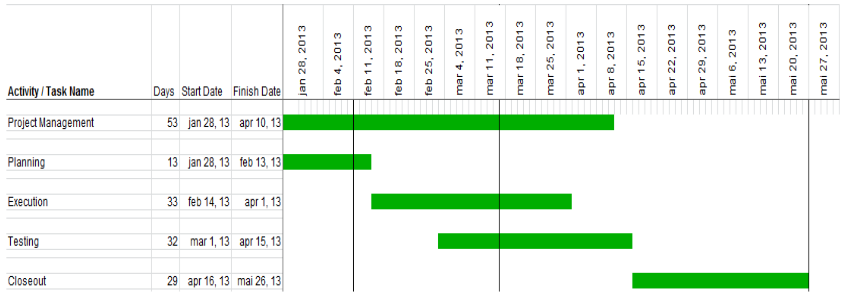
\includegraphics[scale=0.8]{images/gantt-diagram.png}
\caption{Gantt diagram. Milestones are marked using vertical lines}
\end{figure}

\section{Risk analysis}
The risk analysis states risks identified by the team. The importance of a risk is calculated by multiplying likelihood and impact. Higher number means higher importance for the project. 
\captionof{table}{Risk analysis}
\label{fig:risktable}
\begin{longtable}{|m{0.15 \textwidth}|m{0.1 \textwidth}|m{0.1 \textwidth}|m{0.1 \textwidth}|m{0.185 \textwidth}|m{0.185 \textwidth}|}
\hline
	\rowcolor{Gray}
	\textbf{Description} & \textbf{Likeli{-}hood} & \textbf{Impact} & \textbf{Impor{-}tance} & \textbf{Preventive\newline Action} & \textbf{Remedial\newline Action}\\
	\endfirsthead%
	\multicolumn{6}{l}%
	{{\bfseries Continued from previous page}} \\ \hline
	\rowcolor{Gray}
	\textbf{Description} & \textbf{Likeli{-}hood} & \textbf{Impact} & \textbf{Impor{-}tance} & \textbf{Preventive\newline Action} & \textbf{Remedial\newline Action}\\
\hline
	\endhead%
	\hline

	\hline \multicolumn{6}{|l|}{{Continued on next page}} \\ \hline
	\endfoot%

	\endlastfoot%

	Illness & 7 & 2 & 14 & Good\newline communication and effective use of GitHub & Increase workhours and exchange tasks and\newline responsibilities\\
\hline
	Project\newline complexity & 6 & 5 & 30 & Don't take on too much work & Cut down the demands\\
\hline
	Customer\newline issues & 1 & 5 & 5 & Agreement with customer and weekly feedback from customer & Use the\newline original\newline requirement specification\\
\hline
	License\newline incompability & 7 & 7 & 49 & Avoid\newline integrating components with incopatible licenses & Discover other implementations or implment from scratch\\
\hline
	Group\newline conflicts or disagreements & 3 & 3 & 9 & Keep close\newline contact to avoid\newline surprises.\newline Leader takes\newline action & Contact\newline supervisor and make an\newline appointment\\
\hline
	Over the air complexity & 8 & 8 & 64 & Have multiple\newline alternative\newline solutions and keep close\newline contact with customer & Detail what was attempted as well as why it couldn't be solved in the final report.\\
\hline
	Personal matters & 8 & 5 & 40 & Not much\newline preventative action can be taken & Keep in touch and stay\newline updated. In case you still can do tasks, claim one and tell the\newline others\\
\hline
\end{longtable}
